\begin{frame}{Problem Statements}
\begin{columns}
\column{0.5\textwidth}
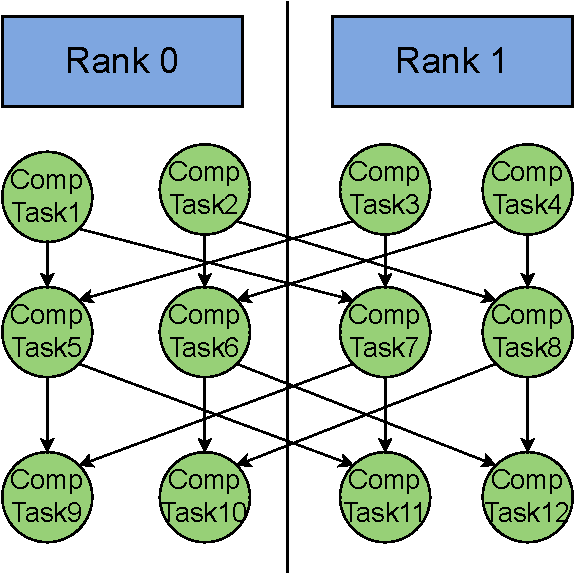
\includegraphics[width=\textwidth]{./Figures/koskelo/cross_hatch.pdf}
\column{0.025\textwidth}
\column{0.475\textwidth}
\alert{Have:} Array DAG, distributed-memory machine

\medskip
\alert{Users Want:} Program execution to be fast

\end{columns}
\end{frame}

\begin{frame}{Current Reality}
    
    \alert{Current implementation:} \didit{Kaushik Kulkarni; M. Smith}
    \begin{itemize}
    \item Each \alert{rank} sends communication nodes $\to$ rank 0 $\to$ \alert{communication graph} (global)
    \item $N$ communication nodes $\to$ batches of communication without intrabatch dependencies
    \begin{itemize}
        \item \alert{minimize} number of communication batches
        \item \completed{} Grouping cost \(O(N^2)\) $\to$ \(O(N)\)
    \end{itemize}
    \item Each \alert{rank} `interweaves' computation into this `schedule skeleton'
    \begin{itemize}
    \item \alert{Fuse} rank local computation nodes in Array DAG $\to$ `parts'
    \item Reorder computation to push communication tasks towards edges of each `part'
    \item Collect `parts' into local `partitions'
    \end{itemize}

    \medskip
    \item Execute `partitions' on each rank
    \item Execute first available part each rank
    \end{itemize}
    
\end{frame}

\begin{frame}{Research Questions}

    \begin{itemize}
        \item \alert{Near term:} Does \alert{minimizing} the number of communication batches in the current reality locally minimize execution time for our system?
        \item Can we reduce execution time by decreasing the sizes of the `parts' to expose more concurrency?
    \end{itemize}
\end{frame}



\begin{frame}{Effect of `Part' Size on Execution Time?}

    \begin{figure}[t!]
        \centering
        \scalebox{0.9}[0.9]{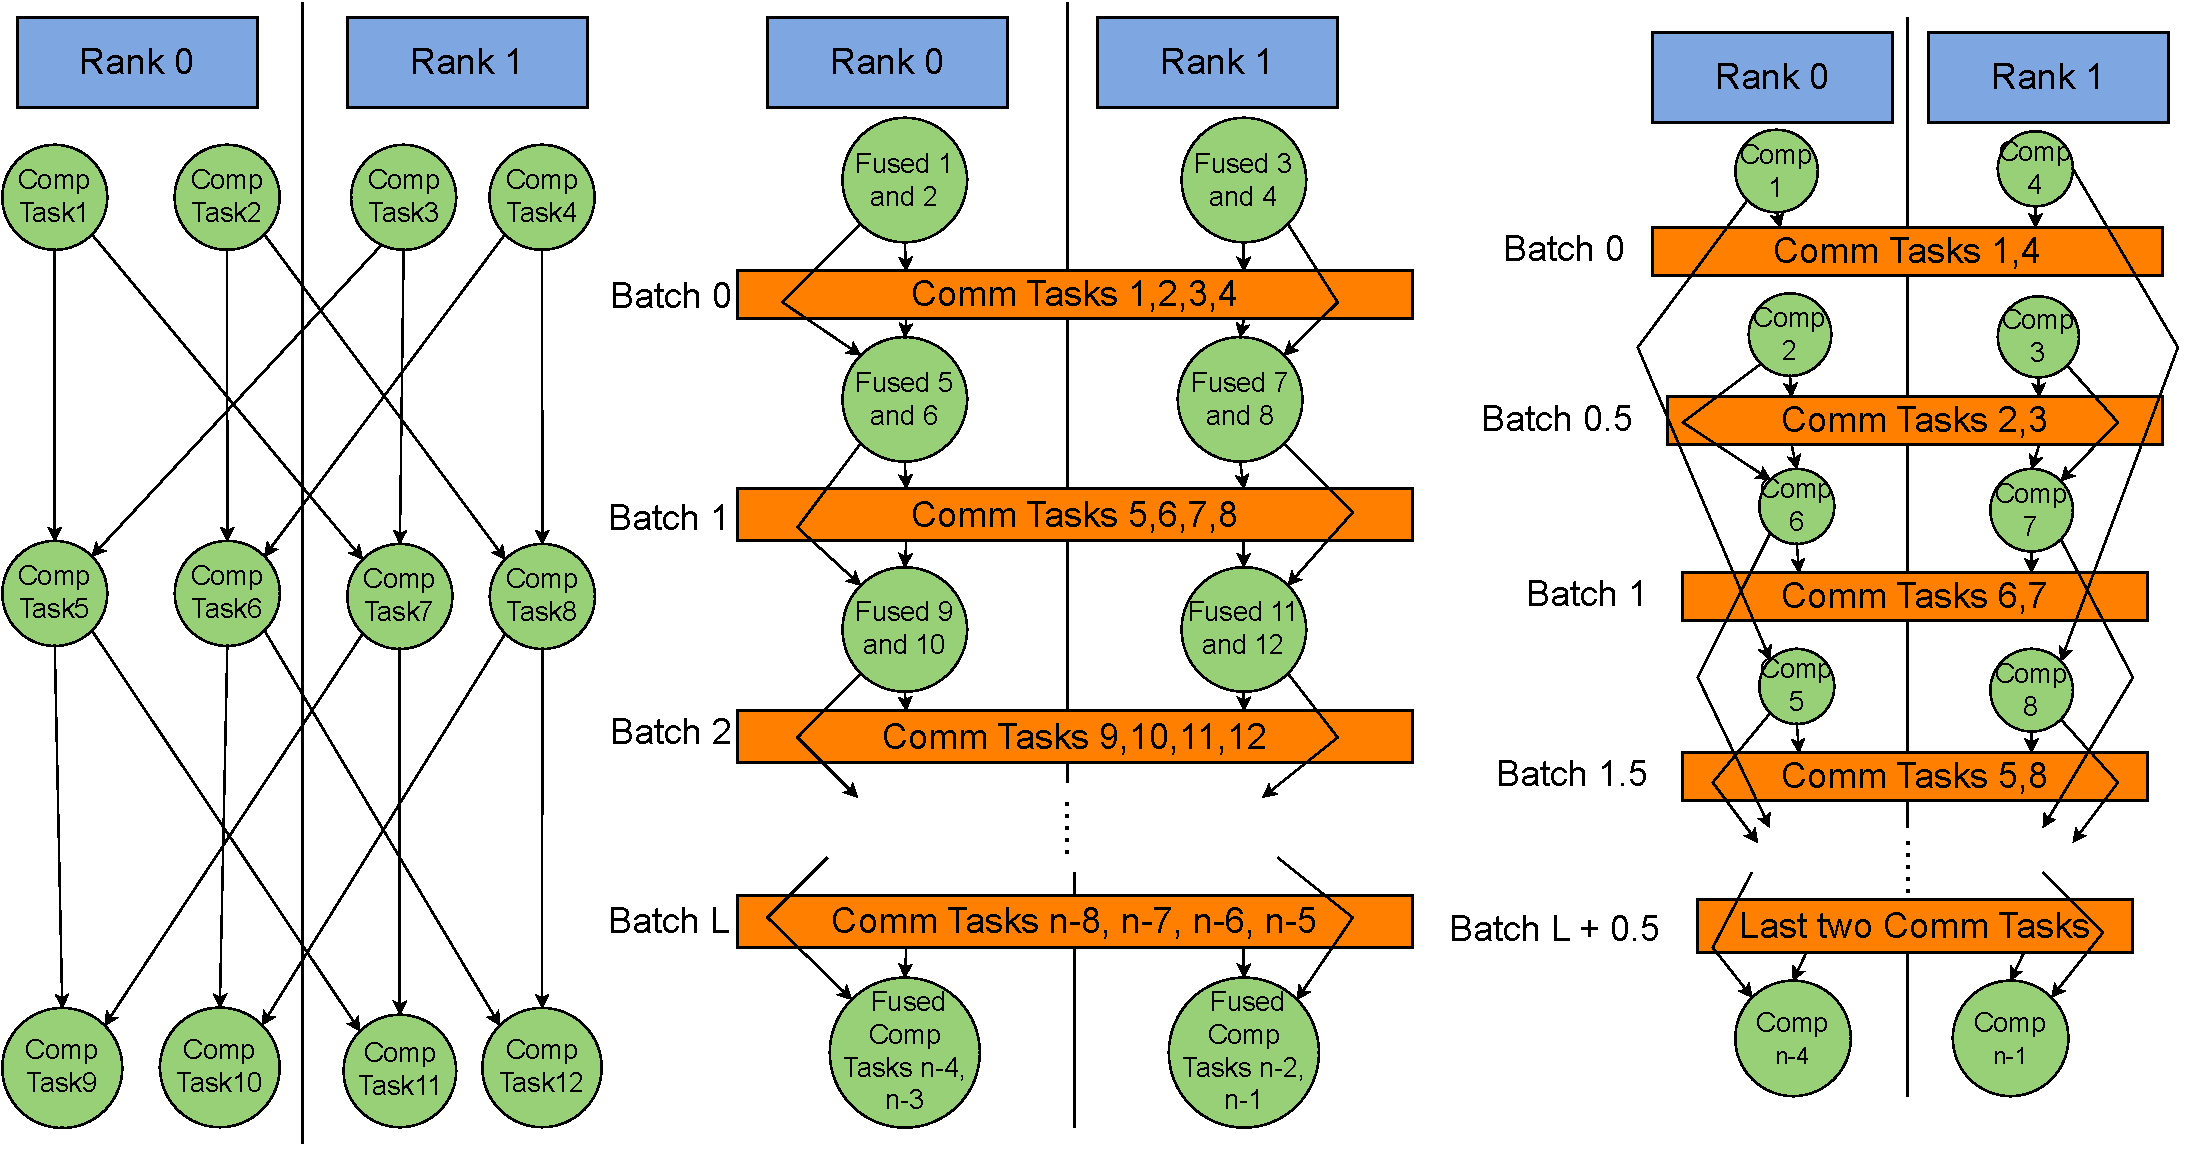
\includegraphics[width=\textwidth]{./Figures/koskelo/cross_hatch_combined.pdf}}
    \end{figure}

\end{frame}

\begin{frame}{Effect of `Part' Size on Execution Time?}

    Experimental Setup
    \begin{itemize}
        \item 2-dimensional wave example in \it{MIRGECOM}
        \item One explicit forward first order Euler time step with 16 elements in each dimension
        \item Workstation with 2 Nvidia Titan-X GPUs
        \item Repeat the test 20 times
    \end{itemize}
    
    \medskip
    Measurements
    \begin{itemize}
        \item Execution Time [s]
        \item Time waiting for communication [s]
    \end{itemize}
\end{frame}    

\begin{frame}{Preliminary Results}
    \begin{tabular}{c|p{3.5cm}|p{3.5cm}|p{2.5cm}|p{2.5cm}}
        Rank & Communication Time Full Batches $(\%)$& Communication Time Half Size Batches $(\%)$  & Execution time Full Levels [s] & Execution Time Half Size Levels [s] \\
        \hline
        0 & $1.5\% \pm 0.28\%$ & $10.5\% \pm 6.5\%$ & $0.264\pm 0.001$ & $1.44 \pm 0.36$ \\
        1 & $0.46\% \pm 0.091\%$ & $27.8\% \pm 6.0\%$ & $0.262\pm 0.0008$ & $1.67 \pm 0.36$ \\
    \end{tabular}

\medskip
\begin{itemize}
    \item \alert{average $\pm$ standard error} on 20 tests
    \item Half Size tests
    \begin{itemize}
        \item 4 of 20 tests, one rank waited $>90\%$ of the execution time
        \item 1 of 20 tests, both ranks waited less than average of full size tests 
    \end{itemize}
\end{itemize}
    \bigskip
    
\begin{itemize}
    \item Splitting the batches in half \alert{increases} the time waiting
    \item Splitting the batches in half \alert{increases} the execution time
    \item \alert{Next step:} improve splitting decision process
\end{itemize}
\end{frame}

